\documentclass[11pt]{beamer}
\usefonttheme[onlymath]{serif}

\setbeamersize{text margin left=1.5em}
\setbeamersize{text margin right=1.5em}

\setbeamertemplate{frametitle}{%
  \vskip1ex
  \usebeamerfont{frametitle}%
  \insertframetitle\par
  \vskip1ex
  \hrule
}

\setbeamertemplate{blocks}[rounded][shadow=true]

\setbeamertemplate{itemize item}{\usebeamerfont{itemize item}\textbullet}
\setbeamertemplate{itemize subitem}{\usebeamerfont{itemize subitem}\textbullet}
\setbeamertemplate{itemize subsubitem}{\usebeamerfont{itemize subsubitem}\textbullet}

\makeatletter
\geometry{%
  papersize={\fpeval{\beamer@paperwidth*1.5}pt,\fpeval{\beamer@paperheight*1.5}pt},
  hmargin=\fpeval{0.5 * 1.5}cm,% 1cm
  vmargin=0cm,%
  head=\fpeval{0.5*1.5}cm,% 0.5cm
  headsep=0pt,%
  foot=\fpeval{0.5*1.5}cm% 0.5cm
}
\makeatother

\usepackage{graphicx}
\usepackage{amsmath}
\usepackage{amssymb}
\usepackage{mathtools}

% Your custom commands (kept as is)
\newcommand{\mrm}[1]{\mathrm{#1}}
\newcommand{\mbb}[1]{\mathbb{#1}}
\newcommand{\mb}[1]{\mathbf{#1}}
\newcommand{\mc}[1]{\mathcal{#1}}
\newcommand{\tb}[1]{\textbf{#1}}

\title{Stabilizing Off-Policy Q-Learning via Bootstrapping Error Reduction (BEAR)}
\author{Gwanwoo Choi}
\institute{MLIC}
\date{} % To use the current date

\begin{document}

\begin{frame}
    \titlepage
\end{frame}

\begin{frame}{Sources of Suboptimality in Offline RL}
    \begin{block}{Distribution-Constrained Operators}
        Given a set of policies $\Pi$, the \tb{distribution-constrained backup operator} is defined as
        \[
            \mc{T}^\Pi Q(s,a) \coloneqq \mbb{E}[R(s,a) + \gamma \mbb{E}_{P(s^\prime|s,a)}[V(s^\prime)]] \quad V(s) \coloneqq \max_{\textcolor{red}{\pi \in \Pi}} \mbb{E}_{\pi}[Q(s,a)]
        \]

        This backup operator converges to a fixed point with similar manner of Q Learning convergence.
    \end{block}

    \vspace{0.5cm}
    When learning from a fixed dataset, two primary sources of error can lead to a suboptimal final policy.

    \begin{block}{1. Suboptimality Bias}
        The set of candidate policies, $\Pi$, that the algorithm considers might be too restrictive.
        \begin{itemize}
            \item If the true optimal policy, $\pi^*$, is not contained within $\Pi$, the best policy we can possibly find is inherently suboptimal from the start.
            \item This error arises from the \tb{limited expressiveness} of the policy set.
        \end{itemize}
    \end{block}

    \begin{block}{2. Distributional Shift}
        The policies used for Bellman backups (derived from $\Pi$) can differ significantly from the data-collection policy, $\beta$.
        \begin{itemize}
            \item This mismatch leads to querying the values of Out-of-Distribution (OOD) actions.
            \item This results in \tb{extrapolation errors} which are then amplified through the bootstrapping process, as seen in Figure 2.
        \end{itemize}
    \end{block}
\end{frame}


\begin{frame}{Formalizing the Error Components: $\alpha(\Pi)$ and $C(\Pi)$}
    We can quantify these two error sources with the following definitions.

    \begin{block}{Suboptimality Constant: $\alpha(\Pi)$}
        \[ \alpha(\Pi) \coloneqq \max_{s,a} |\mc{T}^\Pi Q^*(s,a) - TQ^*(s,a)| = \max_{s,a} |\mc{T}^\Pi Q^*(s,a) - Q^*(s,a)| \]
        \begin{itemize}
            \item It captures the maximum difference between the standard Bellman operator ($\mc{T}Q^*$) and an operator constrained to policies in $\Pi$ ($\mc{T}^\Pi Q^*$).
            \item A \tb{larger, more expressive $\Pi$} leads to a \tb{smaller $\alpha(\Pi)$}.
        \end{itemize}
    \end{block}

    \begin{block}{Concentrability Coefficient: $C(\Pi)$}
        Let $\rho_0$ denote the initial state distribution and $\mu(s,a)$ denote the distribution of training data over $\mc{S}\times \mc{A}$, with marginal $\mu(s)$ over $\mc{S}$.
        Suppose there exists coefficients $c(k)$ such that for any $\pi_1, \dots, \pi_k \in \Pi$ and $s \in \mc{S}$:
        \[ \rho_0 P^{\pi_1} \dots P^{\pi_k}(s) \le c(k) \mu(s) \implies \frac{\rho_0 P^{\pi_1}\dots P^{\pi_k}(s)}{\mu(s)} \leq c(k)\]

        This measures the effect of distributional shift, based on the assumption.
        \begin{itemize}
            \item It bounds the ratio between the state distribution generated by policies in $\Pi$ and the dataset's state distribution $\mu$.
            \item $C(\Pi)$ is a weighted sum of these mismatch coefficients, $c(k)$. A \tb{larger, more diverse $\Pi$} can lead to a \tb{larger $C(\Pi)$}.
            \[
                C(\Pi) \coloneqq (1-\gamma)^2 \sum_{k=1}^\infty k \gamma^{k-1} c(k)
            \]
        \end{itemize}
    \end{block}
\end{frame}

\begin{frame}{The Overall Performance Bound (Theorem 4.1)}
    \begin{columns}[T]
        \begin{column}{.5\textwidth}
            \begin{block}{Shrinking the policy set $\Pi$}
                (e.g., similar to behavior policy)
                \begin{itemize}
                    \item $C(\Pi) \downarrow$ (Safety $\uparrow$)
                    \item $\alpha(\Pi) \uparrow$ (Optimality $\downarrow$)
                \end{itemize}
            \end{block}
        \end{column}
        \begin{column}{.5\textwidth}
            \begin{block}{Expanding the policy set $\Pi$}
                (e.g., considering all policies)
                \begin{itemize}
                    \item $C(\Pi) \uparrow$ (Safety $\downarrow$)
                    \item $\alpha(\Pi) \downarrow$ (Optimality $\uparrow$)
                \end{itemize}
            \end{block}
        \end{column}
    \end{columns}

    \vspace{0.5cm}
    Following theorem combines both error sources to provide an upper bound on the final policy's suboptimality.

    \begin{block}{The Suboptimality Bound}
        Suppose we run approximate distribution-constrained value iteration with a set constrained backup $\mc{T}^\Pi$.
        Assume that $\delta(s,a) \geq \max_k |Q_k(s,a) - \mc{T}^\Pi Q_{k-1} (s,a)|$ bounds the bellman error. Then
        \[
        \lim_{k \to \infty} \mbb{E}_{\rho_0}[|V^{\pi_k}(s) - V^*(s)|] \le \frac{\gamma}{(1-\gamma)^2} \left( \textcolor{red}{C(\Pi) }\mbb{E}_{\mu} [\max_{\pi \in \Pi} \mbb{E}_{\pi}[\delta(s,a)]] + \frac{1-\gamma}{\gamma} \textcolor{red}{\alpha(\Pi)} \right)
        \]
    \end{block}
    
    \begin{itemize}
        \item The \tb{left-hand side} is the final suboptimality gap we want to minimize.
        \item The \tb{right-hand side} shows that the total error depends on two key terms.
    \end{itemize}


    \begin{center}
        \tb{To guarantee good performance, an algorithm must balance keeping $C(\Pi)$ small with keeping $\alpha(\Pi)$ small.}
    \end{center}

    \vspace{1mm}
    \begin{center}
        \tb{Goal: Find an optimal policy set $\Pi$ that minimizes $\alpha(\Pi)$ while keeping $C(\Pi)$ bounded.}
    \end{center}
\end{frame}

\begin{frame}{Theorem 4.2}

    \begin{block}{Support Set}
        \[
            \Pi_{\epsilon} \coloneqq \{\pi | \pi(a|s) =0 \text{ whenever } \beta(a|s) < \epsilon\}
        \]

        \begin{itemize}
            \item By adjusting $\epsilon$, we can control the trade-off between $C(\Pi_\epsilon)$ and $\alpha(\Pi_\epsilon)$.
        \end{itemize}
    \end{block}
    \begin{block}{Theorem 4.2}
        Assume the data distribution $\mu$ is generated by a behavior policy $\beta$.
        Let $\mu(s)$ be the marginal state distribution under the data distribution and $\mu_{\Pi_\epsilon}$ be the \tb{highest discounted marginal state distribution} starting from the initial state distribution $\rho$ and following policies $\pi \in \Pi_\epsilon$ at each time step thereafter.
        Then, there exists a concentrability coefficient $C(\Pi_\epsilon)$ which is bounded:
        \[
            C(\Pi_{\epsilon}) \leq C(\beta) \cdot \left(1 + \frac{\gamma}{(1-\gamma)f(\epsilon)}(1-\epsilon)\right)
        \]
        where $f(\epsilon) \coloneqq \min_{s \in \mc{S} \text{ s.t. } \mu_{\Pi_\epsilon}(s)>0}[\mu(s)]>0$.
    \end{block}
    \begin{itemize}
        \item $f(\epsilon)$ is the lowest probability of any state in the support of $\mu_{\Pi_\epsilon}$.
    \end{itemize}
\end{frame}


\begin{frame}{Visualizing the Core Problem: Error Propagation (Fig. 2)}
    \begin{columns}[T] % Divide the frame into columns
        
        % Left Column for the Figure
        \begin{column}{0.5\textwidth}
            \begin{figure}
                \centering
                % --- Please insert Figure 2 from the BEAR paper here ---
                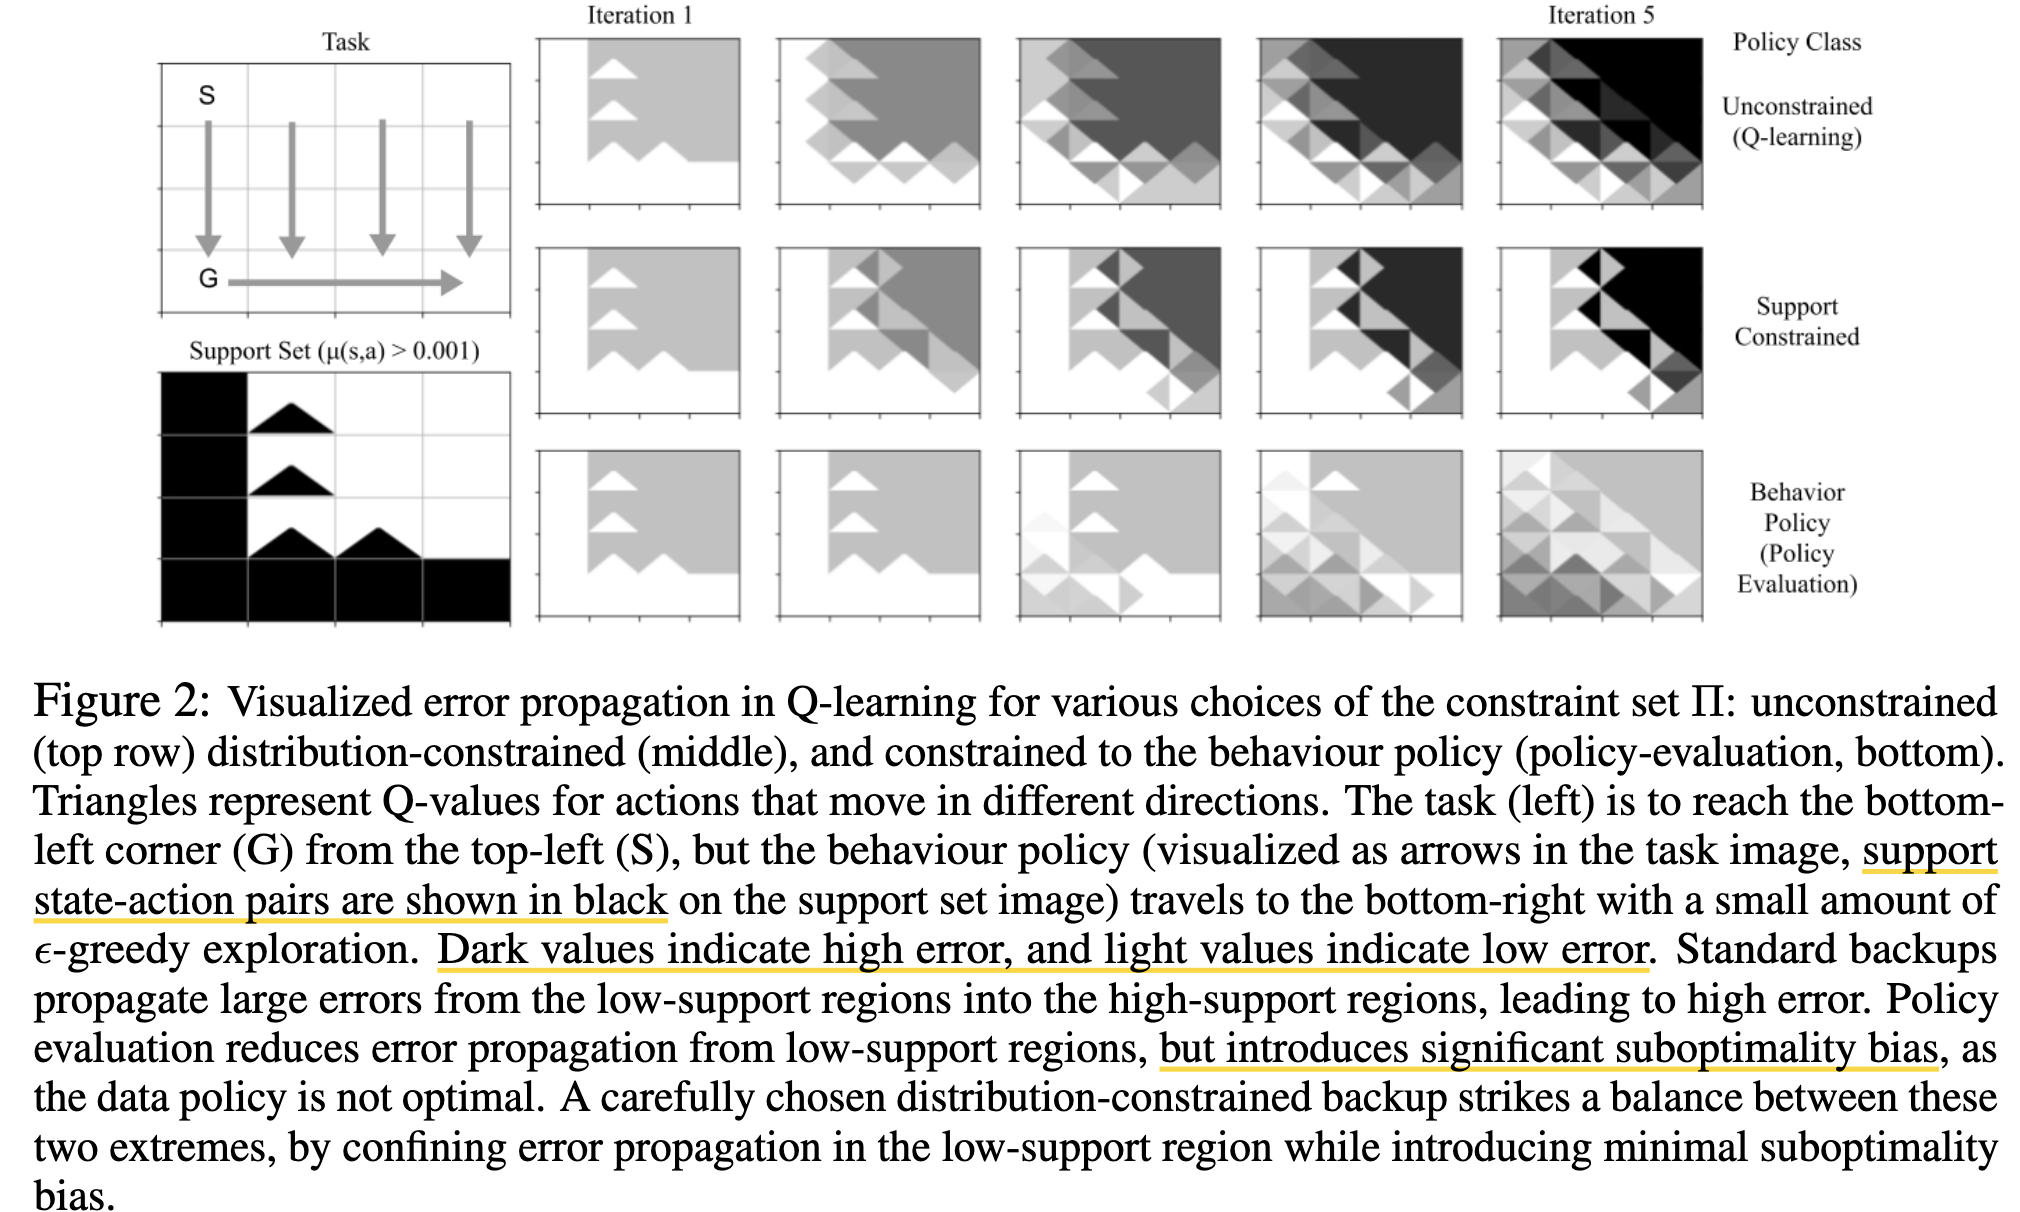
\includegraphics[width=\textwidth]{Figure2.png}
                \caption{Error propagation in a gridworld.}
            \end{figure}
        \end{column}
        
        % Right Column for the Explanation
        \begin{column}{0.5\textwidth}
            \begin{itemize}
                \item \tb{Setup}: The data is collected by a policy moving away from the optimal goal, creating an Out-of-Distribution (OOD) region with high initial error (top-right).
                \vspace{1em}
                \item \tb{Unconstrained (Q-learning)}: Fails. The $\max$ operator propagates high error from the OOD region into the data-supported region, corrupting the Q-values.
                \vspace{1em}
                \item \tb{Behavior Policy (Policy Eval.)}: Stable but suboptimal. It avoids error propagation but cannot learn a better policy.
                \textcolor{magenta}{Why the error propagation starts from the goal state?}
                \vspace{1em}
                \item \tb{Support Constrained ($\Pi_\epsilon$)}: It strikes a balance by confining error propagation to the OOD region while allowing for stable policy improvement.
            \end{itemize}
        \end{column}
        
    \end{columns}
\end{frame}

\begin{frame}{BEAR: Core Idea and Components}
    \begin{block}{Core Idea}
        Explicitly constrain the learned policy to lie within the \tb{support} of the behavior policy's data distribution.
        \begin{itemize}
            \item "Search for the optimal policy only within the realm of actions the data has shown us."
            \item This prevents $C(\Pi)$ from exploding, thus avoiding error accumulation.
        \end{itemize}
    \end{block}

    \begin{block}{Key Components}
        \begin{enumerate}
            \item \tb{Ensemble of Q-functions}: Learn multiple Q-functions and use the minimum value for conservative estimation, enhancing stability.
            \item \tb{MMD-based Support Constraint}: Since the behavior policy $\beta$ is unknown, use a sample-based distance metric, Maximum Mean Discrepancy (MMD), to ensure the learned policy $\pi$ stays close to $\beta$.
        \end{enumerate}
    \end{block}
\end{frame}

\begin{frame}{Ensemble of Q-functions}
    \begin{block}{Ensemble of Q-functions}
        \begin{itemize}
            \item Train $K$ independent Q-functions, $\{\hat{Q}_1, \hat{Q}_2, \dots, \hat{Q}_K\}$.
            \item Use the minimum of these Q-values for policy improvement:
            \[ \min_{j=1,..,K} \hat{Q}_j(s,a) \]
            \item The policy is updated to maximize the conservative estimate of the Q-values within $\Pi_\epsilon$:
            \[\pi_\phi (s) \coloneqq \max_{\pi \in \Pi_\epsilon} \mbb{E}_{a \sim \pi(\cdot|s)}\left[ \min_{j=1,\dots,K} \hat{Q}_j(s,a)\right]\]
            \item This conservative estimate helps mitigate overestimation bias and provides a more robust value function.
        \end{itemize}
    \end{block}
\end{frame}

\begin{frame}{The MMD (Maximum Mean Discrepancy) Constraint}
    \begin{itemize}
        \item \tb{Problem}: We cannot directly use the theoretical constraint ($\pi(a|s)=0 \text{ if } \beta(a|s)<\epsilon$) because the true distribution of $\beta$ is unknown.
        \item \tb{Solution}: Use MMD, which can compute the distance between two distributions using only samples.
    \end{itemize}
    
    \begin{block}{Constrained Policy Update Objective}
    \begin{align*}
    \pi_\phi := \max_{\pi} \quad & \mbb{E}_{s \sim \mc{D}, a \sim \pi(\cdot|s)} \left[ \min_{j=1,..,K} \hat{Q}_j(s,a) \right] \\
    \text{s.t.} \quad & \mbb{E}_{s \sim \mc{D}} \left[ \text{MMD}(\mc{D}(s), \pi(\cdot|s)) \right] \leq \epsilon
    \end{align*}
    \end{block}

    \begin{itemize}
        \item \tb{Objective}: Maximize the conservative expectation of the Q-value.
        \item \tb{Constraint}: The MMD distance between the learned policy $\pi$ and the data distribution $\mc{D}$ must not exceed a threshold $\epsilon$.
    \end{itemize}
\end{frame}

\begin{frame}{ALgorithms}
    \begin{block}{Constrained Policy Update Objective}
        \begin{align*}
            \pi_\phi := \max_{\pi} \quad & \mbb{E}_{s \sim \mc{D}, a \sim \pi(\cdot|s)} \left[ \min_{j=1,..,K} \hat{Q}_j(s,a) \right] \\
            \text{s.t.} \quad & \mbb{E}_{s \sim \mc{D}} \left[ \text{MMD}(\mc{D}(s), \pi(\cdot|s)) \right] \leq \epsilon
        \end{align*}
    \end{block}
    \begin{figure}
        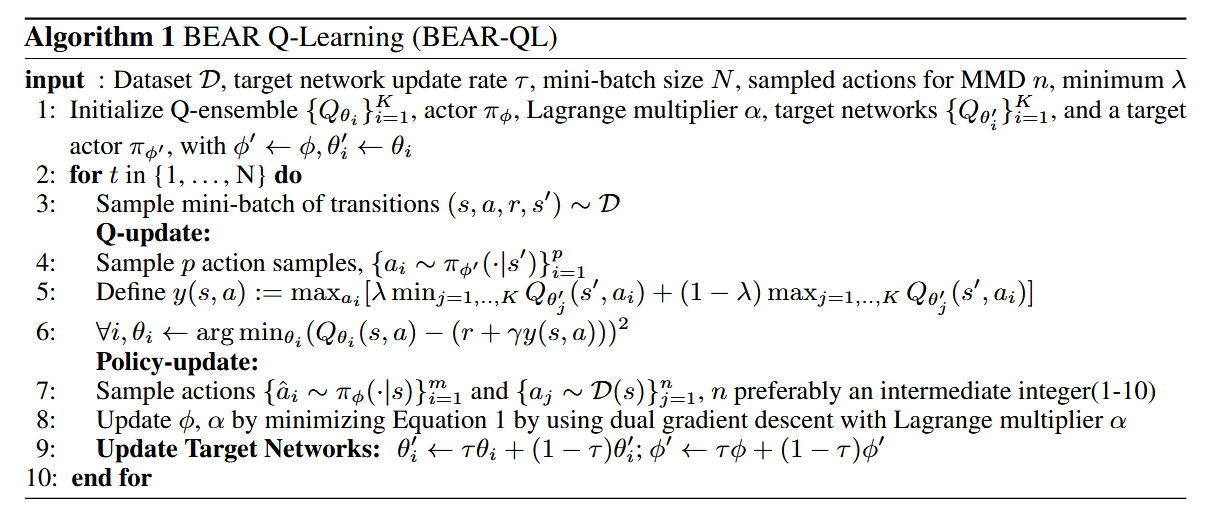
\includegraphics[width=0.94\textwidth]{Algorithm.png}
    \end{figure}
\end{frame}

\begin{frame}{Experiment: Baselines}
    \begin{block}{Baselines}
        \begin{itemize}
        \item Off-Policy \tb{TD3}
        \item \tb{BCQ}
        \item \tb{KL-control} (BCQ + KL-constraint)
        \item (static version of ) \tb{DQfD}
        \item \tb{BC} (Behavior Cloning)
        \end{itemize}
    \end{block}

    \begin{block}{Plot}
        \begin{itemize}
            \item \tb{X-axis} : number of gradient updates taken by each algorithm. One step on the x-axis corresponds to 1000 gradient steps.
            \item \tb{Y-axis} : average evaluation return over 5 seeds of the policy
        \end{itemize}
    \end{block}
\end{frame}

\begin{frame}{Experiment 1: Performance on Medium-Quality Data}
    \begin{itemize}
        \item The most realistic scenario: data collected from a partially trained, imperfect policy.
        \item The magenta dashed line indicates the average performance of the data-collection policy.
    \end{itemize}
    
    \begin{figure}
        \centering
        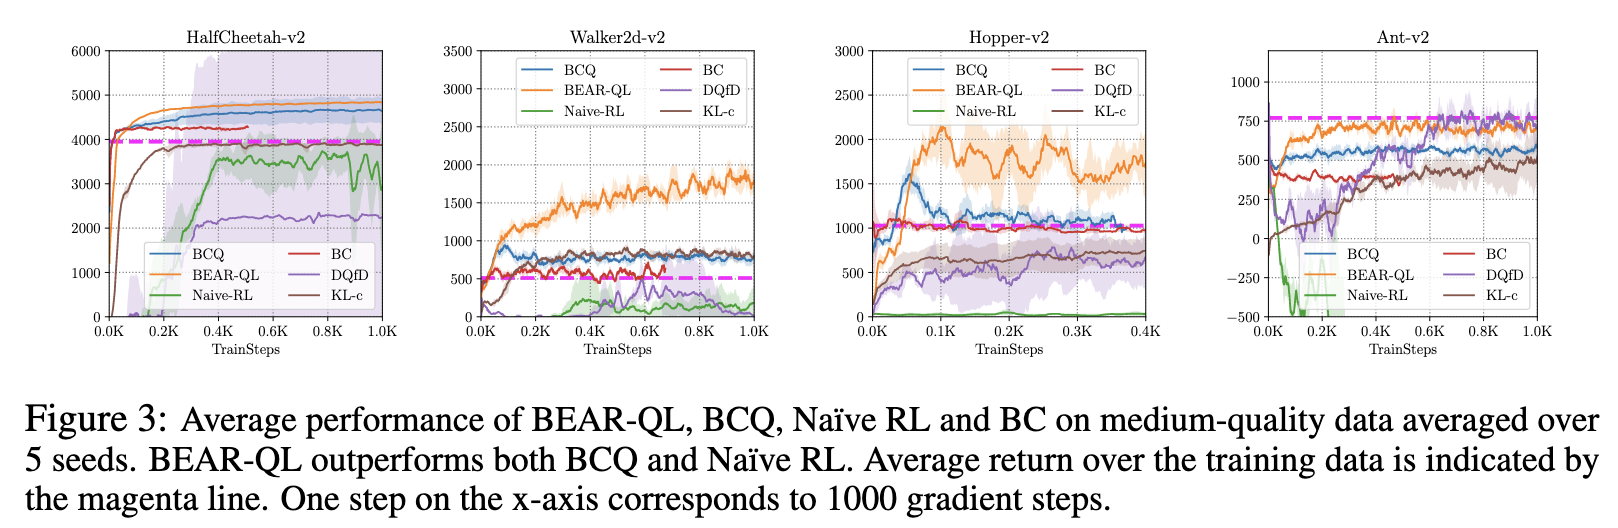
\includegraphics[width=0.9\textwidth]{Figure3.png}
        \caption{Performance on medium-quality data.}
    \end{figure}
    
    \begin{itemize}
        \item \tb{BEAR-QL} consistently outperforms baselines and successfully improves upon the behavior policy.
        \item \tb{BCQ} often tracks the performance of the BC baseline, suggesting that BCQ primarily imitates the data.
        \item \tb{KL-control} usually performs similar or worse to BC
        \item \tb{DQfD} tends to diverge often due to cumulative error due to OOD actions and often exhibits a huge variance across different runs (For example, HalfCheetah-v2 environments)
        \item \tb{Naive-RL} fails to learn and suffers from performance degradation due to error accumulation.
    \end{itemize}
\end{frame}

\begin{frame}{Experiment 1: Performance on Medium-Quality Data (Appendix E)}
    \begin{figure}
        \centering
        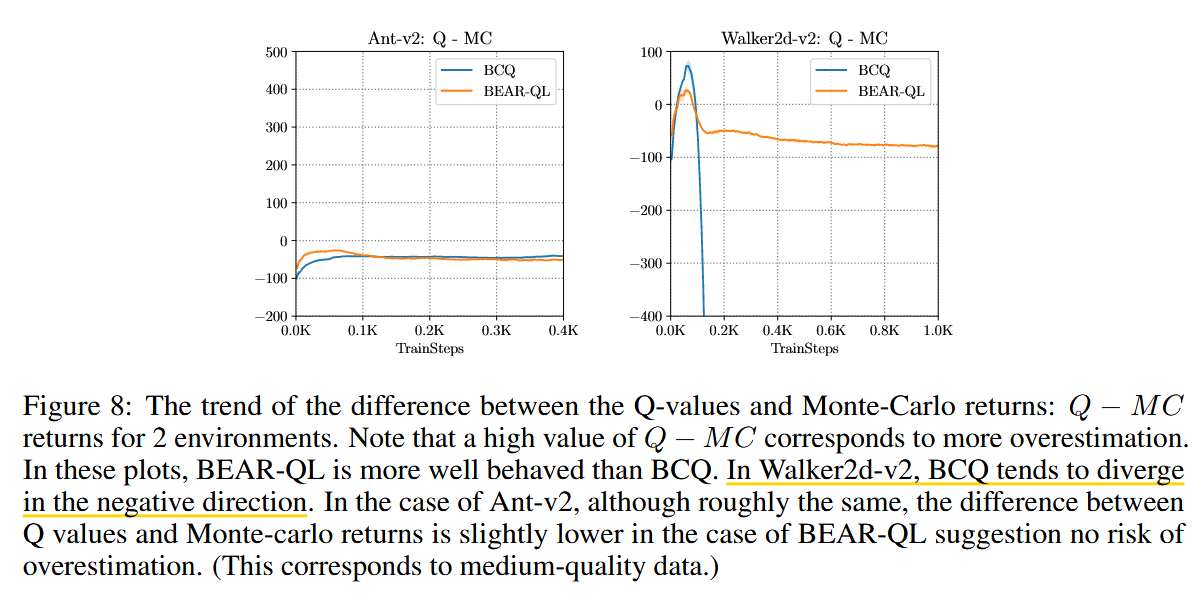
\includegraphics[width=0.6\textwidth]{Figure8.png}
    \end{figure}
    \begin{figure}
        \centering
        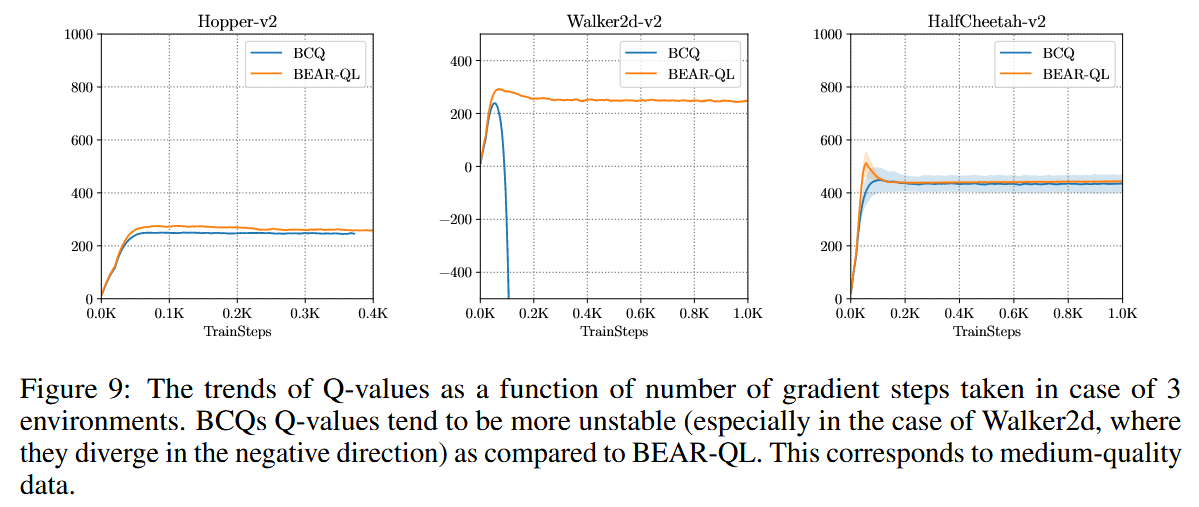
\includegraphics[width=0.6\textwidth]{Figure9.png}
    \end{figure}
        \begin{itemize}
        \item In Figure 8, $Q-MC$ of the policy in the environment are provided
        \item In Figure 9, Q-values learned by BEAR-QL and BCQ are provided.
        \item BCQs Q-values tend to be more unstable (especially, in Walker2d) as compared to BEAR-QL
    \end{itemize}
\end{frame}

\begin{frame}{Experiment 2: Performance on Extreme Datasets}
        \begin{figure}
            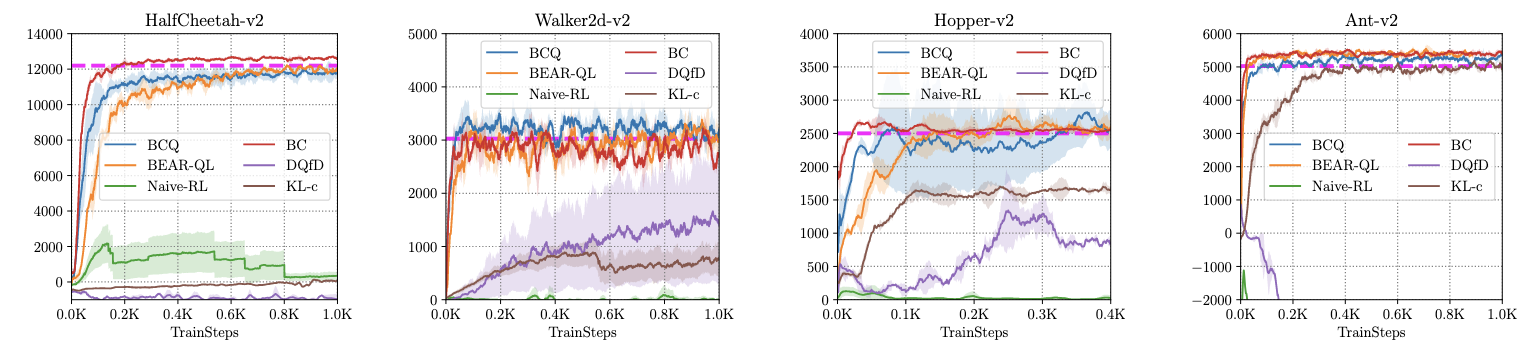
\includegraphics[width=\textwidth]{Figure5Bottom.png}
            \caption{Random Data}
        \end{figure}
        \begin{itemize}
            % \item \tb{Goal}: Test policy \textit{improvement}.
            \item \tb{BEAR, Naive-RL}: BEAR achieves good results, Naive-RL often does well.
            \item \tb{BCQ}: Favors a BC strategy, causing it to fail on random data.
        \end{itemize}
        \begin{figure}
            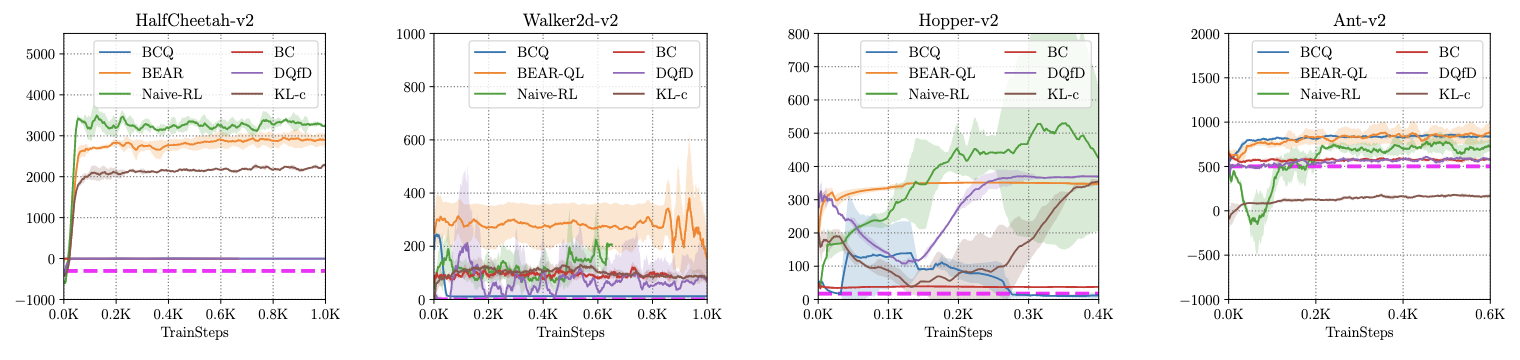
\includegraphics[width=\textwidth]{Figure5Top.png}
            \caption{Optimal Data}
        \end{figure}
        \begin{itemize}
            % \item \tb{Goal}: Test policy \textit{stability}.
            \item \tb{BEAR, BCQ}: Succeed.
            \item \tb{Naive-RL}: Can't handle optimal data, since it doesn't illustrate mistakes.
        \end{itemize}
    \end{frame}

\begin{frame}{Ablation Studies: Validating BEAR's Design}
    \begin{figure}
     % --- Insert Figure 6a ---
     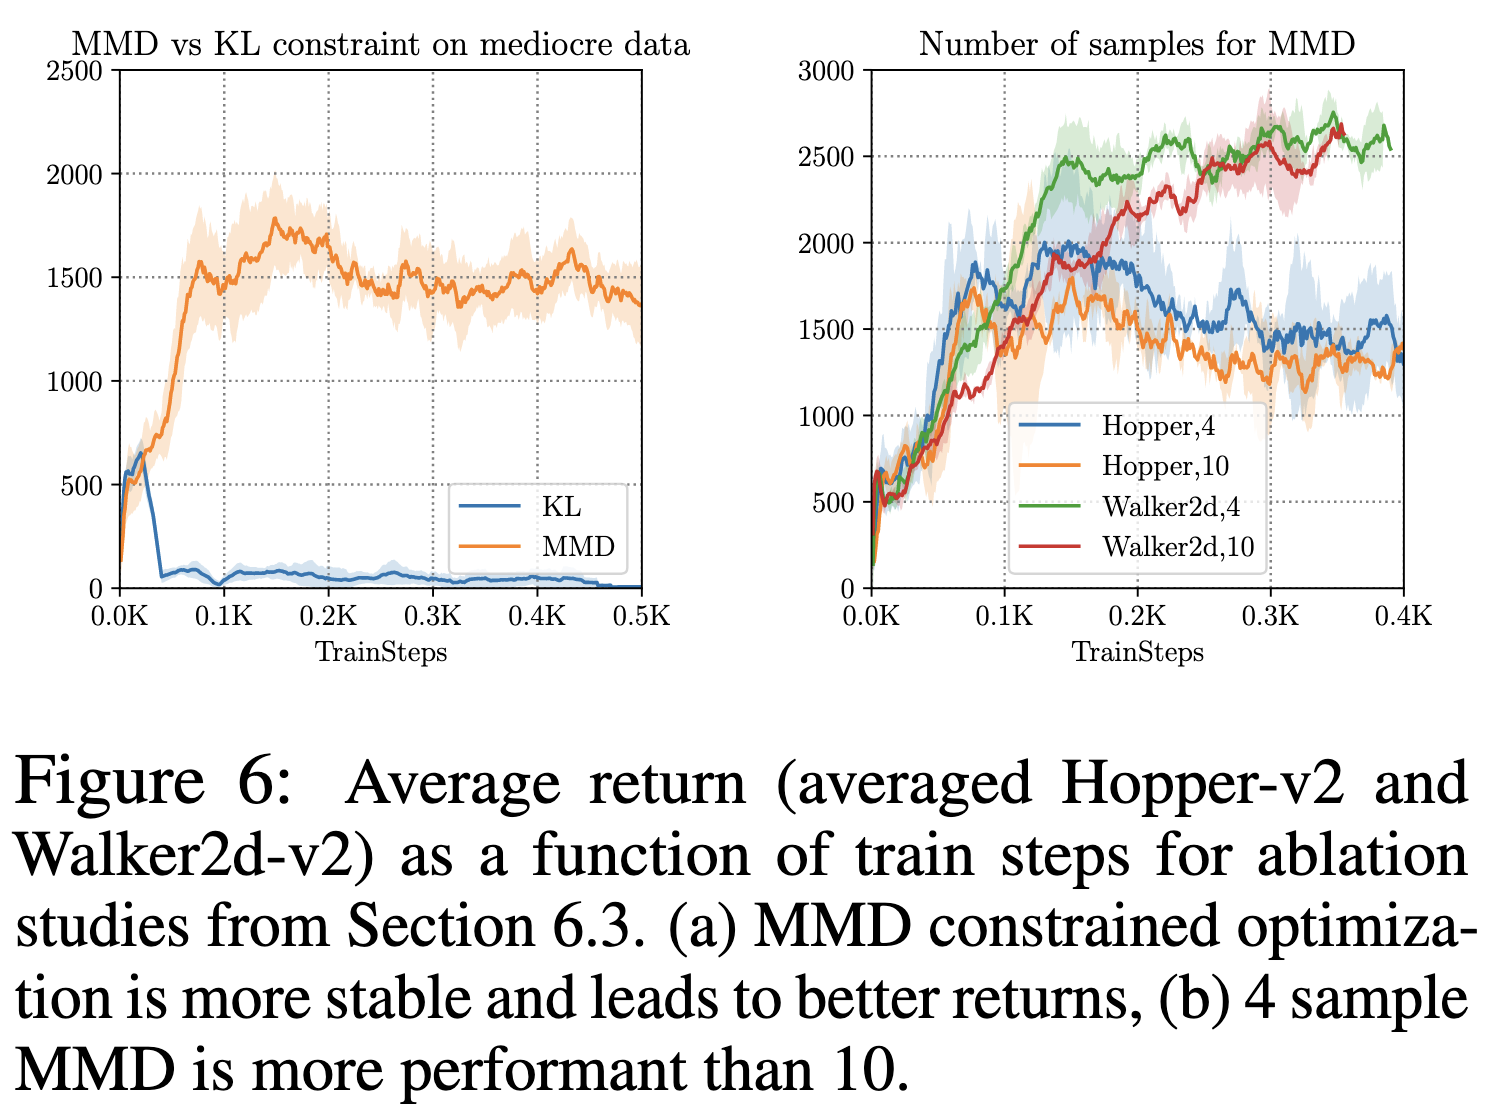
\includegraphics[width=0.5\textwidth]{Figure6.png}
    \end{figure}
    \begin{block}{MMD vs KL-Divergence}
            \begin{itemize}
                \item \tb{Question}: Why use MMD?
                \item \tb{Result}: The KL constraint is too strict (density matching), causing learning to fail in medium-quality data. MMD provides a better balance (support matching).
            \end{itemize}
    \end{block}

    \begin{block}{Number of MMD Samples}
        \begin{itemize}
            \item \tb{Question}: How many samples `n`?
            \item \tb{Result}: A small number of samples (n=4) performs better, likely acting as a form of regularization.
        \end{itemize}
    \end{block}
\end{frame}

\begin{frame}{Experiment 1: Performance on Medium-Quality Data (Appendix E)}
    \begin{figure}
        \centering
        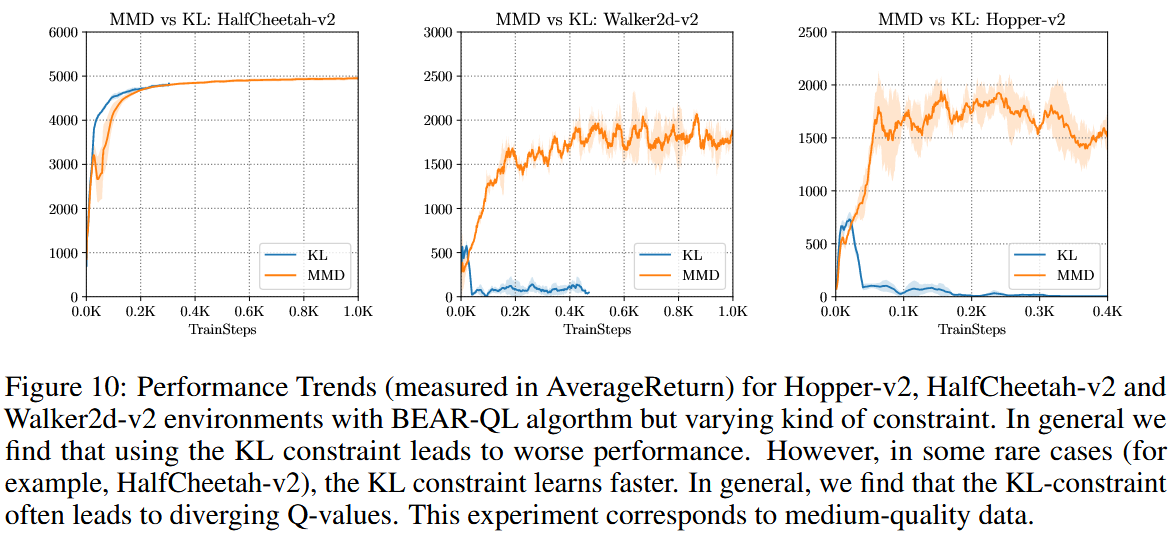
\includegraphics[width=0.6\textwidth]{Figure10.png}
    \end{figure}
    \begin{figure}
        \centering
        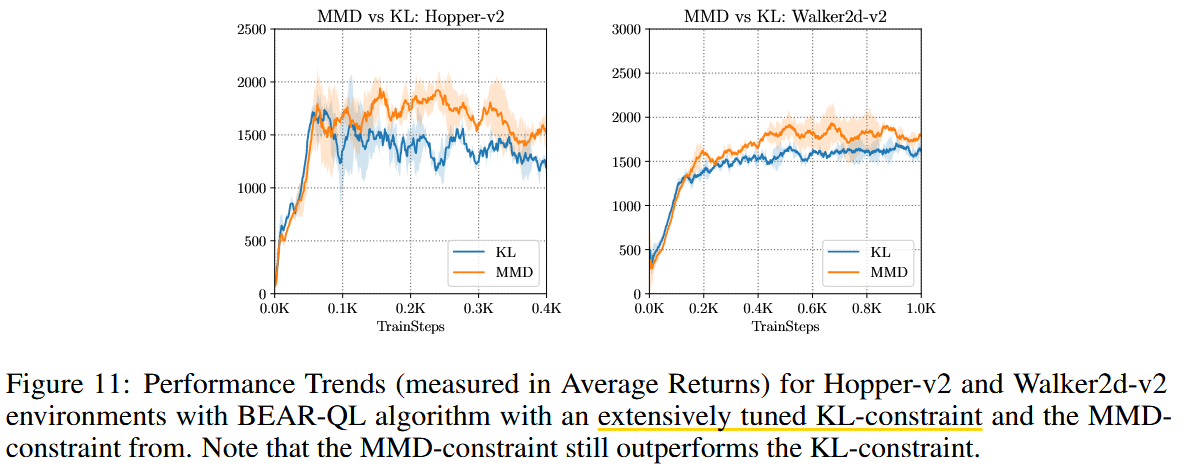
\includegraphics[width=0.6\textwidth]{Figure11.png}
    \end{figure}
    \begin{itemize}
        \item Figure 10 and 11 shows performance trends (mesuared in Average Returns) with using \tb{MMD constraint} vs \tb{KL constraint}
        \item Even in Figure 11, Lagrangian multipler for KL constraint is fine-tuned, MMD constraint shows better performance than KL constraint
    \end{itemize}
\end{frame}

% \begin{frame}{Experiment 1: Performance on Medium-Quality Data (Appendix E)}
%     \begin{figure}
%         \centering
%         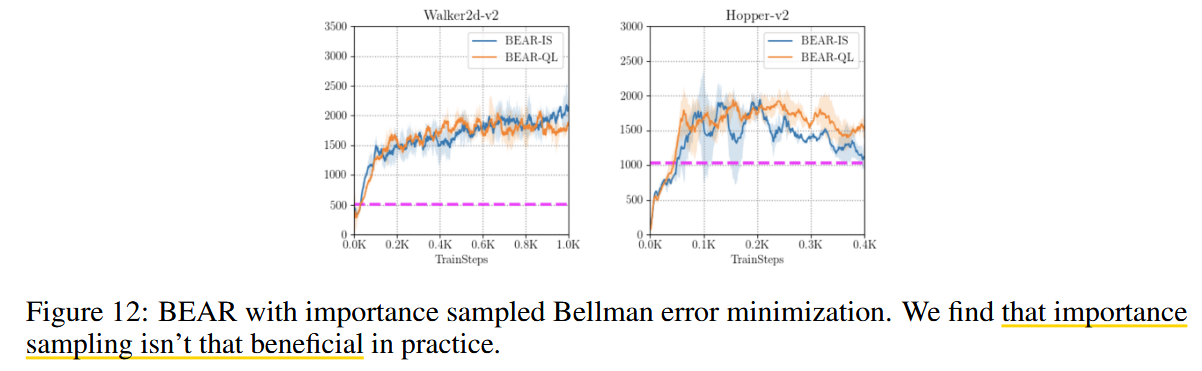
\includegraphics[width=0.7\textwidth]{Figure12.png}
%     \end{figure}
%     How can calculate MMD with importance sampling?
% \end{frame}

\begin{frame}{Discussion}
    \begin{block}{Opinion}
        In my opinion,
        \begin{itemize}
            \item If MMD's performance is as good as the paper claims, why wasn't it mentioned in a later paper like CQL? It looks like MMD and KL divergence seem to have similar performance.
        \end{itemize}
    \end{block}
\end{frame}

\begin{frame}{Appendix: Definition of Maximum Mean Discrepancy}
    \begin{block}{Maximum Mean Discrepancy (MMD)}
        \begin{itemize}
            \item A statistical distance metric that measures the difference between two distributions based on samples.
            \item Given two sets of samples $\{x_i\}_{i=1}^m$ from distribution $P$ and $\{y_j\}_{j=1}^n$ from distribution $Q$, MMD is defined as:
            \[
            \text{MMD}(P, Q) = \left\| \frac{1}{m} \sum_{i=1}^m \phi(x_i) - \frac{1}{n} \sum_{j=1}^n \phi(y_j) \right\|_{\mathcal{H}}
            \]
            where $\phi$ is a feature mapping to a reproducing kernel Hilbert space (RKHS) $\mathcal{H}$.
            \item Intuitively, MMD captures how different the two distributions are by comparing their means in the feature space.
        \end{itemize}
    \end{block}

    \begin{block}{Sampled Maximum Mean DIscrepancy}
        Given samples $x_1, \cdots, x_n \sim P$ and $y_1, \cdots, y_m \sim Q$
        \[
        \text{MMD}^2(X, Y) = \frac{1}{n^2} \sum_{i=1}^n \sum_{j=1}^n k(x_i, x_j) + \frac{1}{m^2} \sum_{i=1}^m \sum_{j=1}^m k(y_i, y_j) - \frac{2}{mn} \sum_{i=1}^n \sum_{j=1}^m k(x_i, y_j)
        \]
        where $k(\cdot,\cdot)$ is any universal kernel function (e.g., Gaussian kernel).
        \begin{itemize}
            \item This empirical estimate allows us to compute MMD using only samples from the distributions, making it practical for our offline RL setting.
        \end{itemize}
    \end{block}
\end{frame}

\end{document}